\documentclass[10pt]{ctexart}
\usepackage{amsmath}
\usepackage{graphicx}
\usepackage{caption}
\title{量子擦除实验报告}
\author{F组}
\begin{document}
\maketitle
\section{实验原理}
\subsection{马赫-曾德尔干涉仪}
马赫-曾德尔干涉仪是一个分波面干涉仪,干涉仪可以通过分束器将单独光源发射的光束分裂成两道准直光束,经过不同路径,最后再次经过分束器汇聚在两个接受屏上,产生干涉条纹.

光强为$I=4I_0\cos^2(\frac{\Delta\phi}{2})$
\subsection{量子物理中的路径信息}
偏振片可以让入射光中只与偏振方向相同的分量出射。

在未放置偏振片时,两条路径上的光子无法区分,因此会在两个接收屏上发生干涉。而在放置了相互垂直的两个偏振片后,两条路径光子的偏振方向不同,于是我们可以通过光子的偏振方向读取其中的路径信息,进而不再存在干涉。

从电磁波的角度,不同方向的电场并不会相互叠加,因此当偏振方向分离后,电场不再相互干涉,光强仅仅正比于两个方向上电场的平方和,不再有干涉条纹出现。
\subsection{量子橡皮擦}
在其中一块接收屏前放置与前两块偏振片成45°的偏振片,这样,路径的信息在到达光屏时再度消失,因为不论光子之前的偏振方向如何,此时光子的偏振方向都只有一个。光子不可区分,在这块接收屏上就发生了干涉。

从电磁学的角度,两个方向垂直的电场经过偏振片方向相同,因此相互叠加,产生条纹。
\section{实验器材}
\begin{itemize}
    \item 532nm激光二极管模块(绿光清晰度高,便于观察)
    \item 1英寸凸透镜,焦距为75mm(选择焦距为7.5厘米,大致是光具组的线度,便于调节产生平行光
    \item 2英寸50:50分束器(让分束器分出的两束平行光光强接近,干涉衬比度更明显;由于有两束光入射在分束镜上,因此将分束镜尺寸制作为2英寸,更方便调节)
    \item 3个1英寸旋转偏振器
    \item 两个1英寸铝镜
    \item 2台屏幕
    \item 校准工具(涉及多次对光路水平、垂直的调节,带有刻度的校准工具可实现这点)
    \item 铝制实验板(除去基础的平台,此实验还使用了双层光学平台来加强稳定性)
\end{itemize}
\begin{minipage}{\textwidth} 
    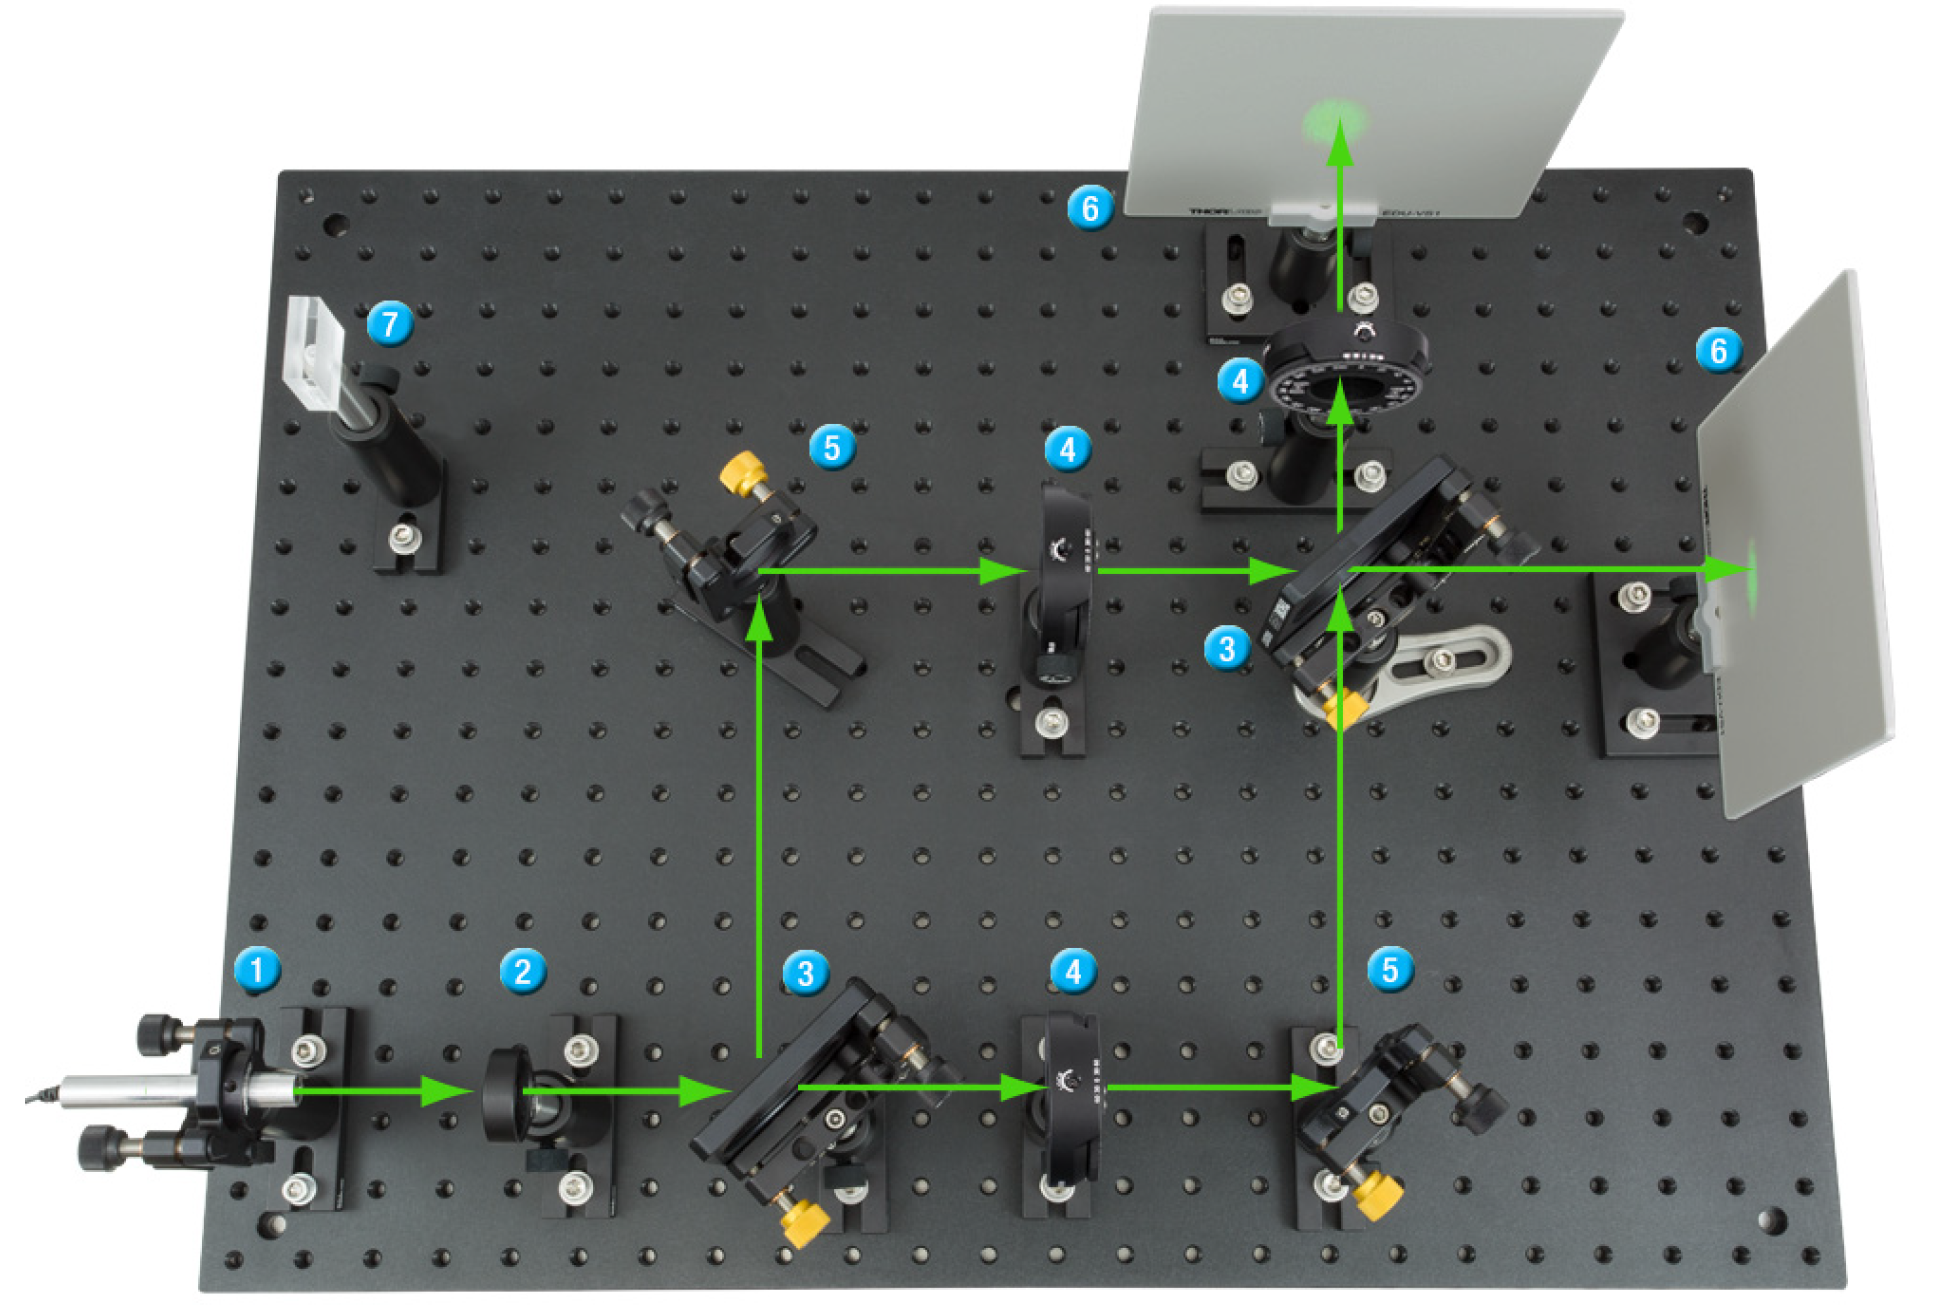
\includegraphics[width=0.8\textwidth]{干涉仪光路图.png}
    \captionof{figure}{干涉仪光路图}
\end{minipage}
\newpage
\section{实验步骤}
\subsection{校准偏光镜}
\begin{itemize}
    \item 将激光器,两偏振片和光屏共线地置于试验板上。转动其中一片偏振片使
    得光屏上实现消光。此时两偏振片垂直,记下两镜角度值;
    \item 将第一个偏光镜组件围绕立柱轴旋转180 度;顺时针旋转第二个偏振镜,直到光屏上再次消光。记下转动第二个偏光镜的角度$\psi$;
    \item 将第一个偏光镜绕立柱轴转回初始时的位置。顺时针转动第一个偏振镜$\frac{\psi}{2}$,再旋转第二个偏光镜使得光屏上消光;
    \item 此时两镜的偏振方向即为一水平一竖直。取下两偏光镜,拧下刻度盘螺丝
    以重新校准偏振角度的零点。使前镜为0 度,后镜为90 度。
\end{itemize}
\subsection{调节干涉仪:}
由于本实验所用激光的相干长度较短,调节难度较大,我们未能在首次实验中调出干涉条纹。以下是我们调节的基本步骤:
\begin{itemize}
    \item 将高度校准工具从
    激光器移至试验板末端,同时观察校准工具上激光点的位置,微调使激光器保持水平;
    \item 放置反射镜,使反射角尽可能接近45度;
    \item 放置分束镜及另一反射镜,并尽可能入射角接近45度;
    \item 在两束光前分别放置校准工具。微调分光镜倾角使得校准物沿试验台前后运动时,激光能始终打在校准物中心;
    \item 放置光屏,另一侧成像与远处的墙面。微调各倾角旋钮,使得两组光斑分别重合;
    \item 放上扩束镜以观察干涉条纹(尽管没观测到)。
\end{itemize}

\begin{minipage}{\textwidth} 
    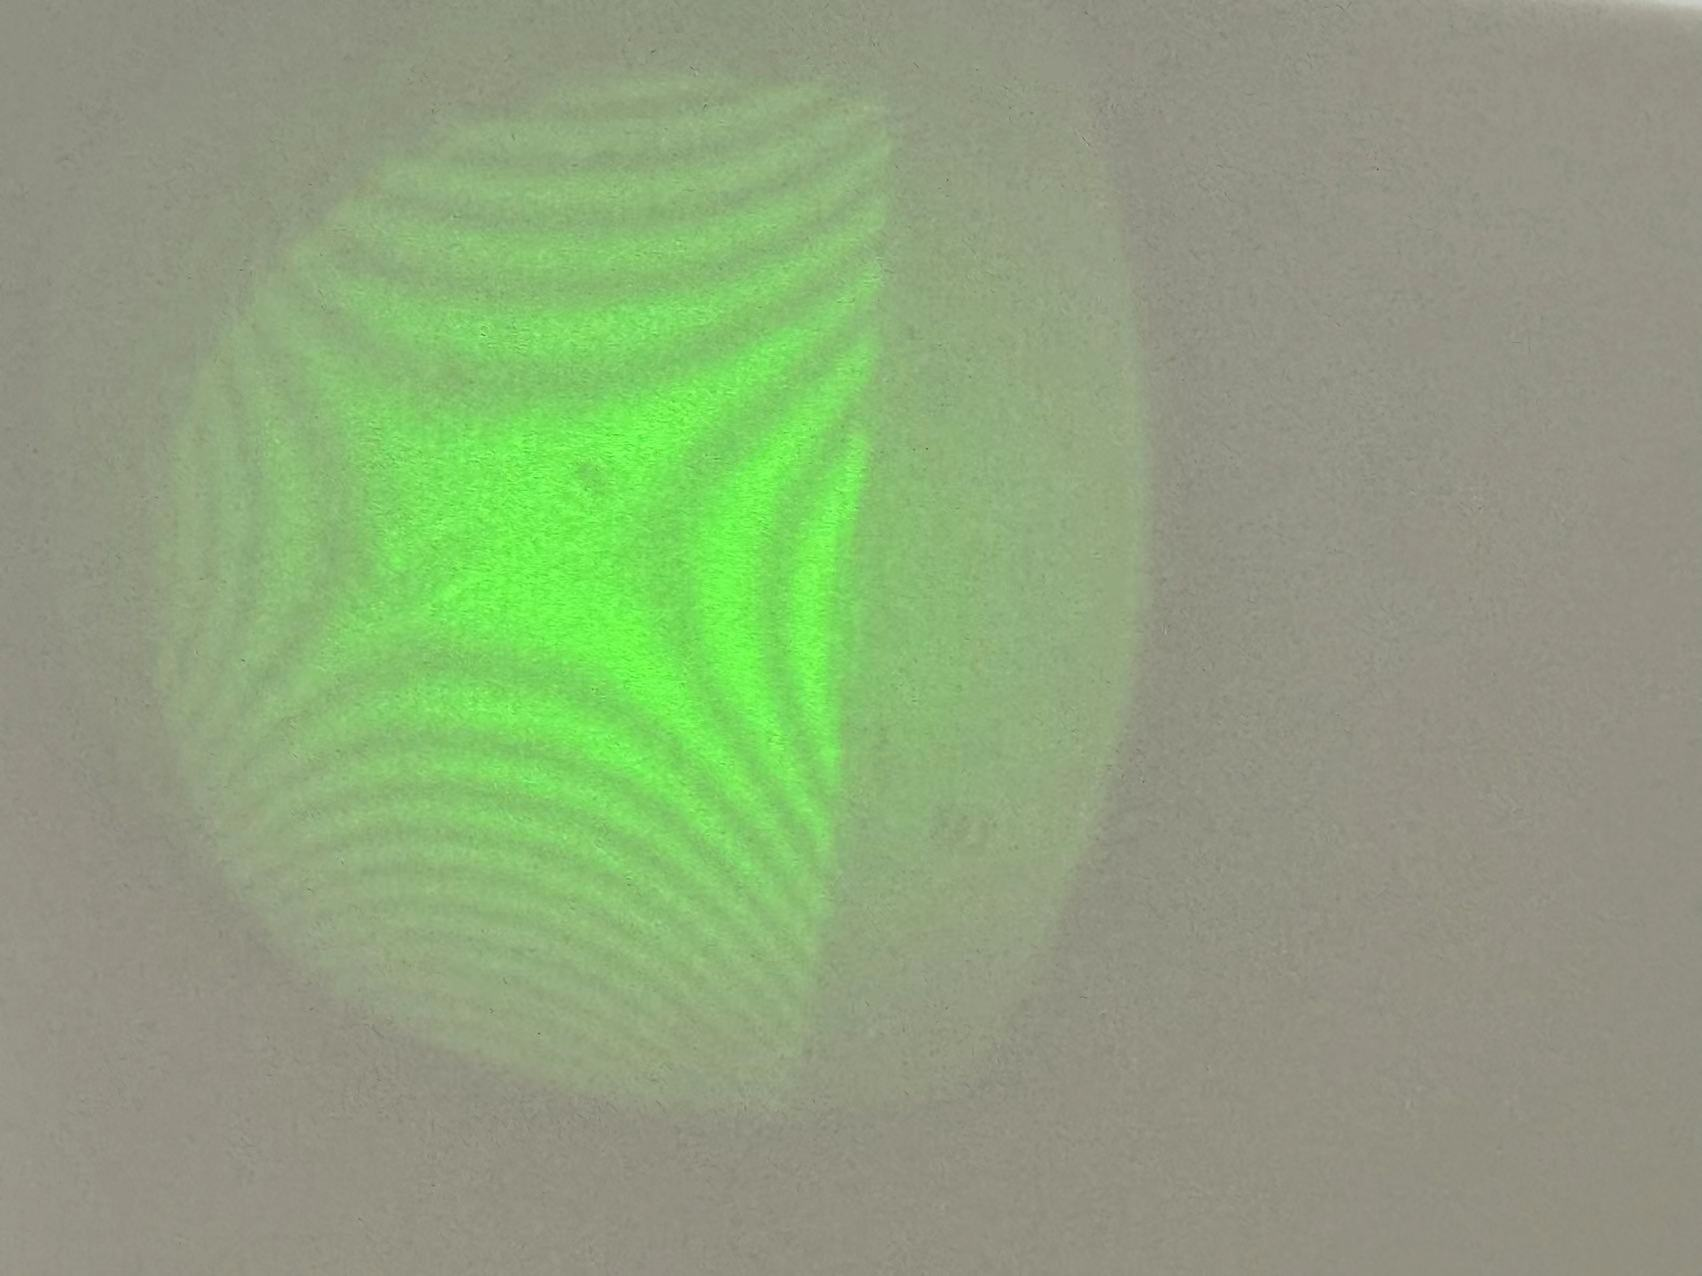
\includegraphics[width=0.8\textwidth]{不加任何偏振片.jpg}
    \captionof{figure}{不加任何偏振片}
\end{minipage}
\begin{minipage}{\textwidth} 
    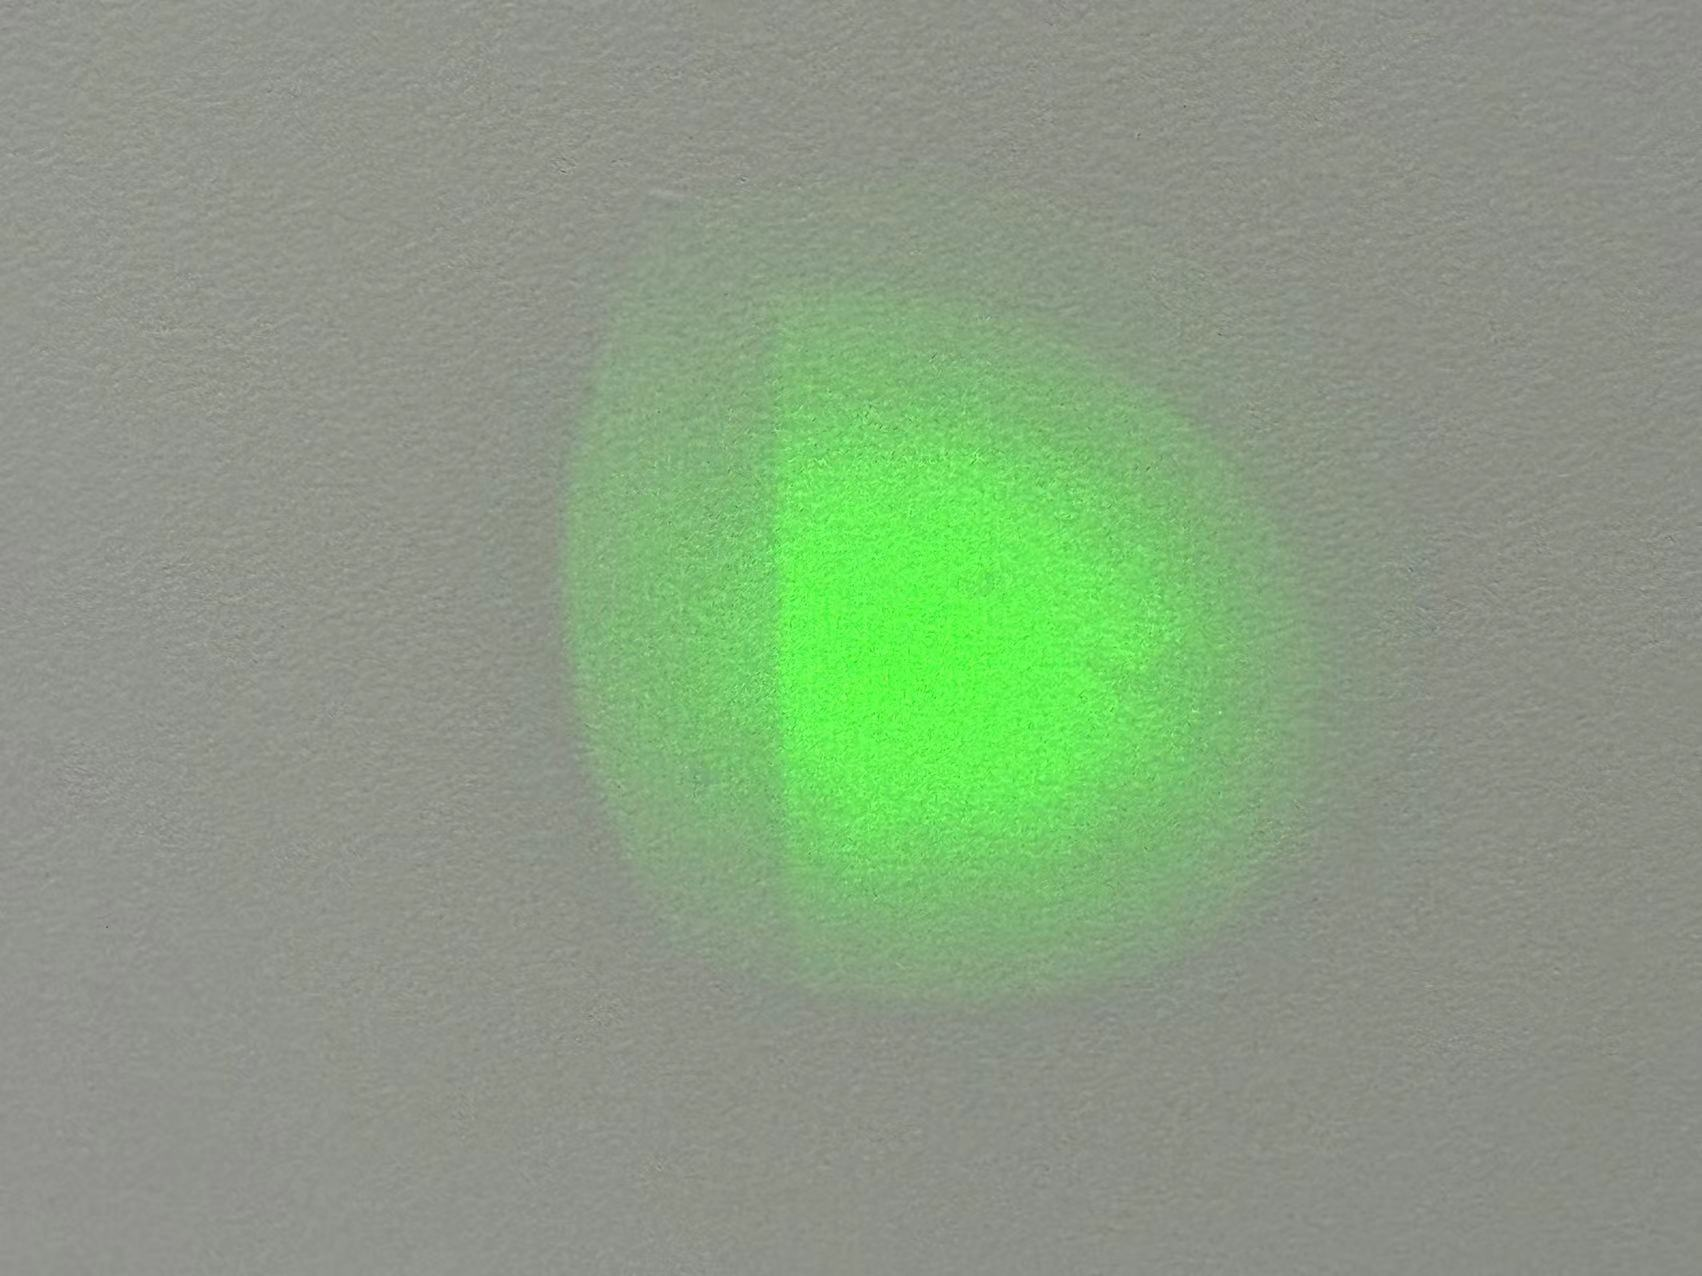
\includegraphics[width=0.8\textwidth]{两边加入偏振方向相互垂直的偏振片后的图像.jpg}
    \captionof{figure}{两边加入偏振方向相互垂直的偏振片后的图像}
\end{minipage}
\begin{minipage}{\textwidth} 
    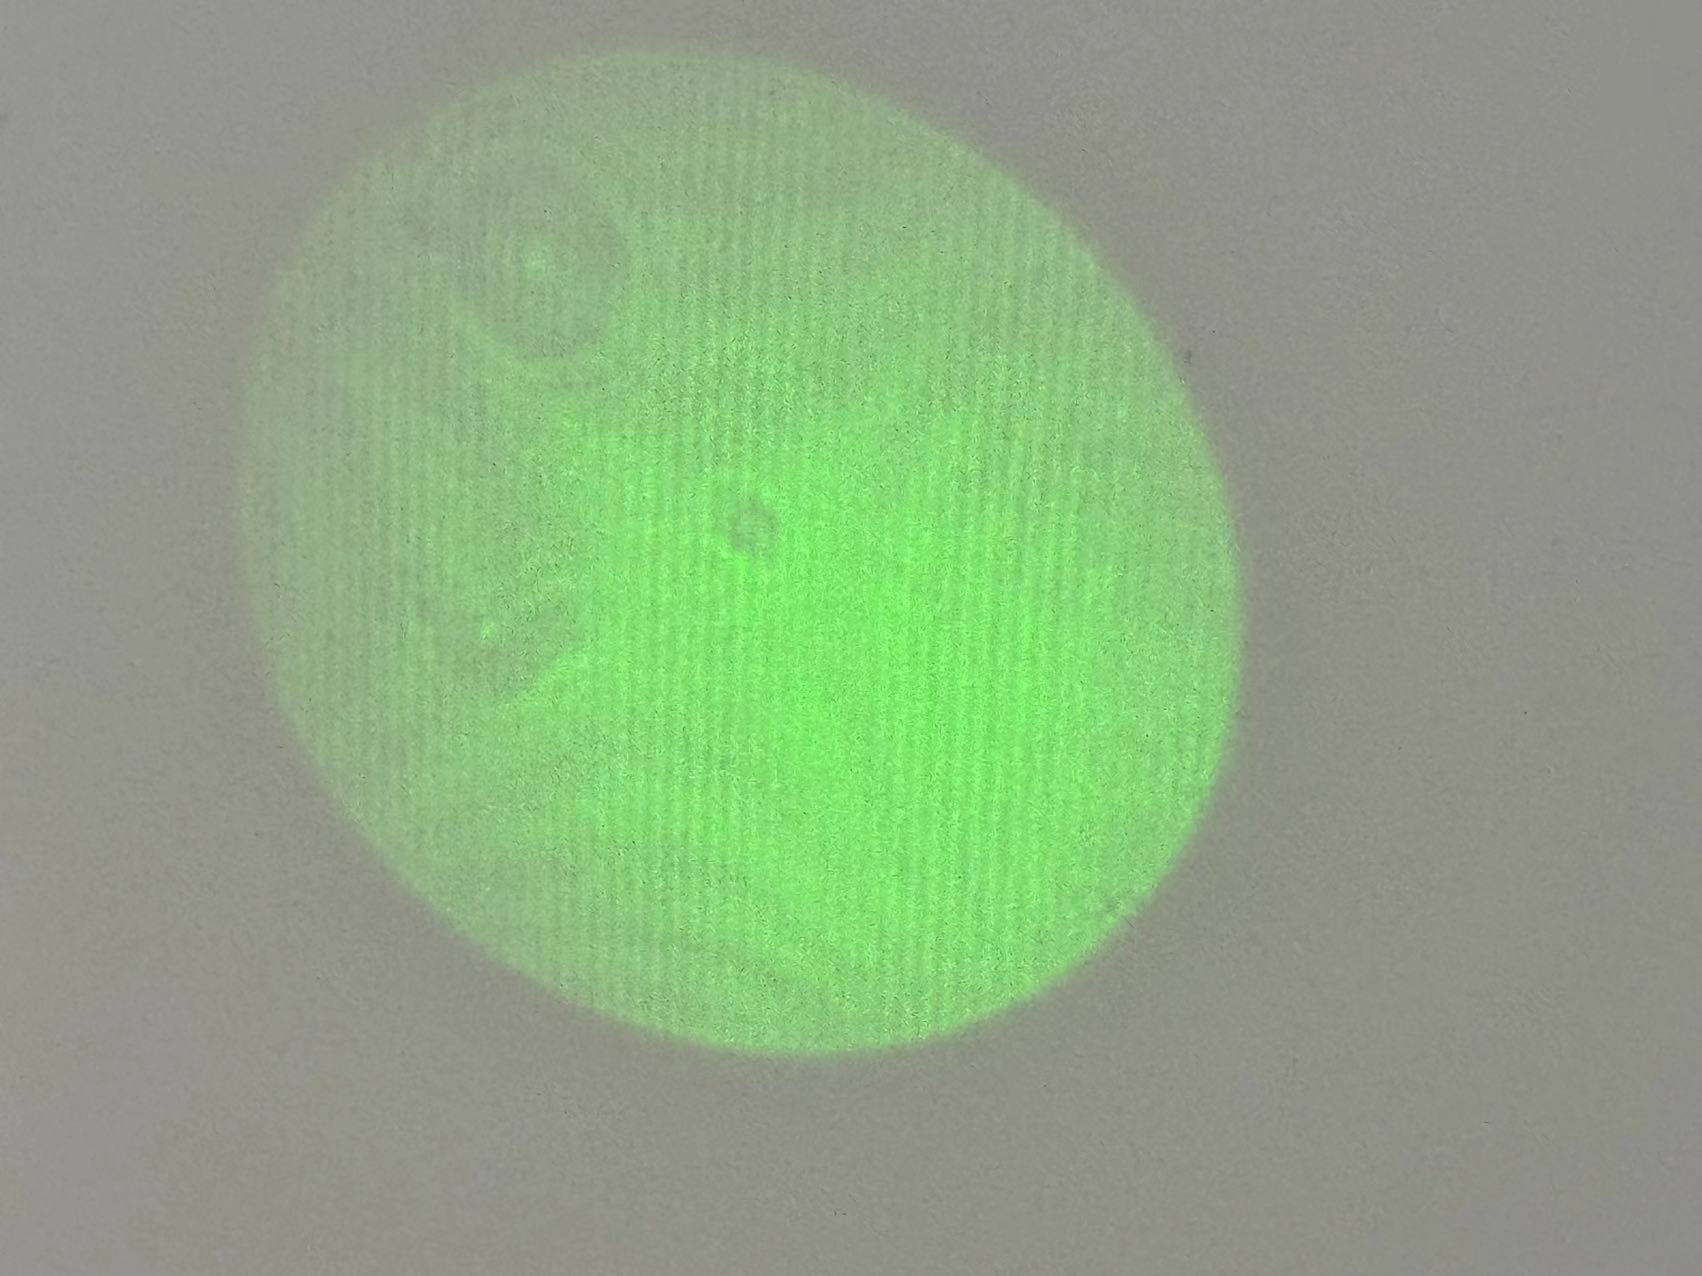
\includegraphics[width=0.8\textwidth]{加入45度偏振片.jpg}
    \captionof{figure}{加入45度偏振片}
\end{minipage}
\begin{minipage}{\textwidth} 
    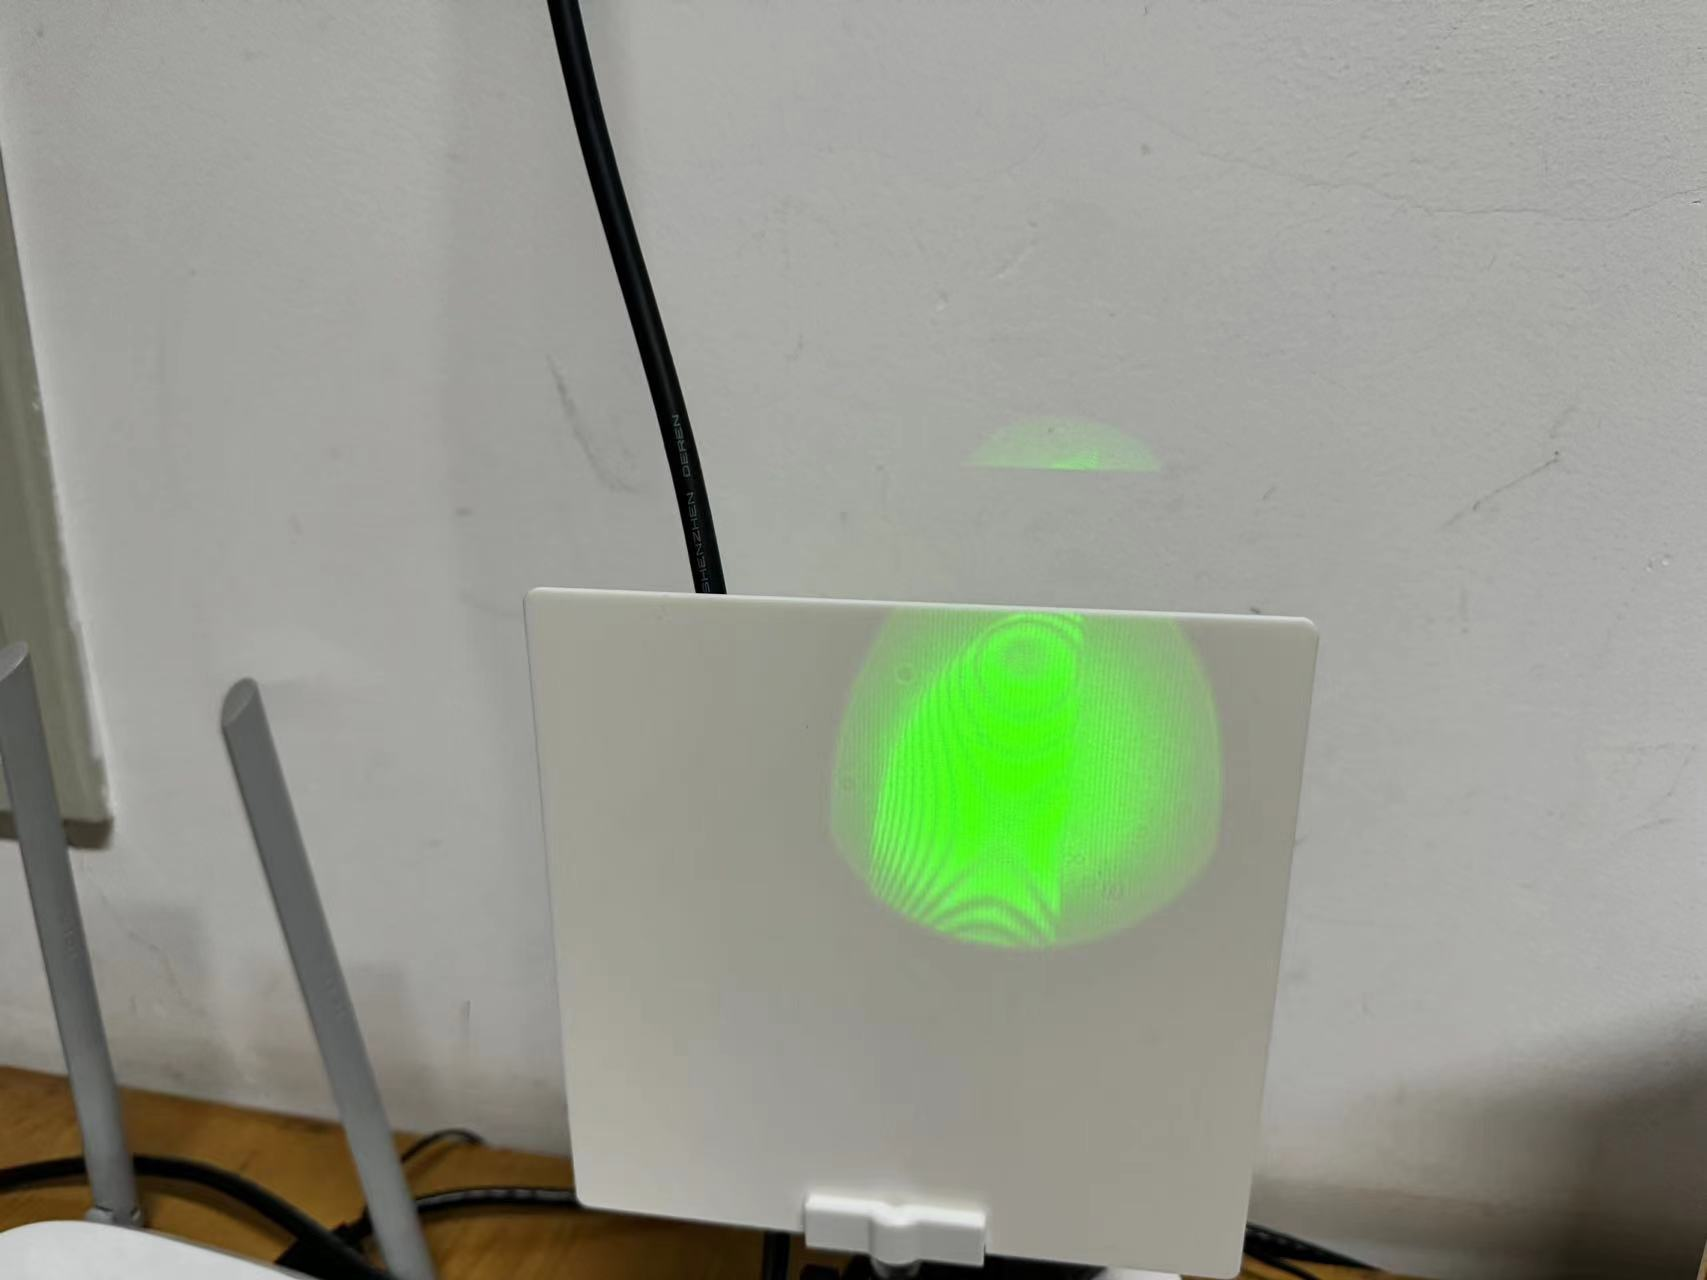
\includegraphics[width=0.8\textwidth]{其一.jpg}
    \captionof{figure}{调出的其他图案}
\end{minipage}
\begin{minipage}{\textwidth} 
    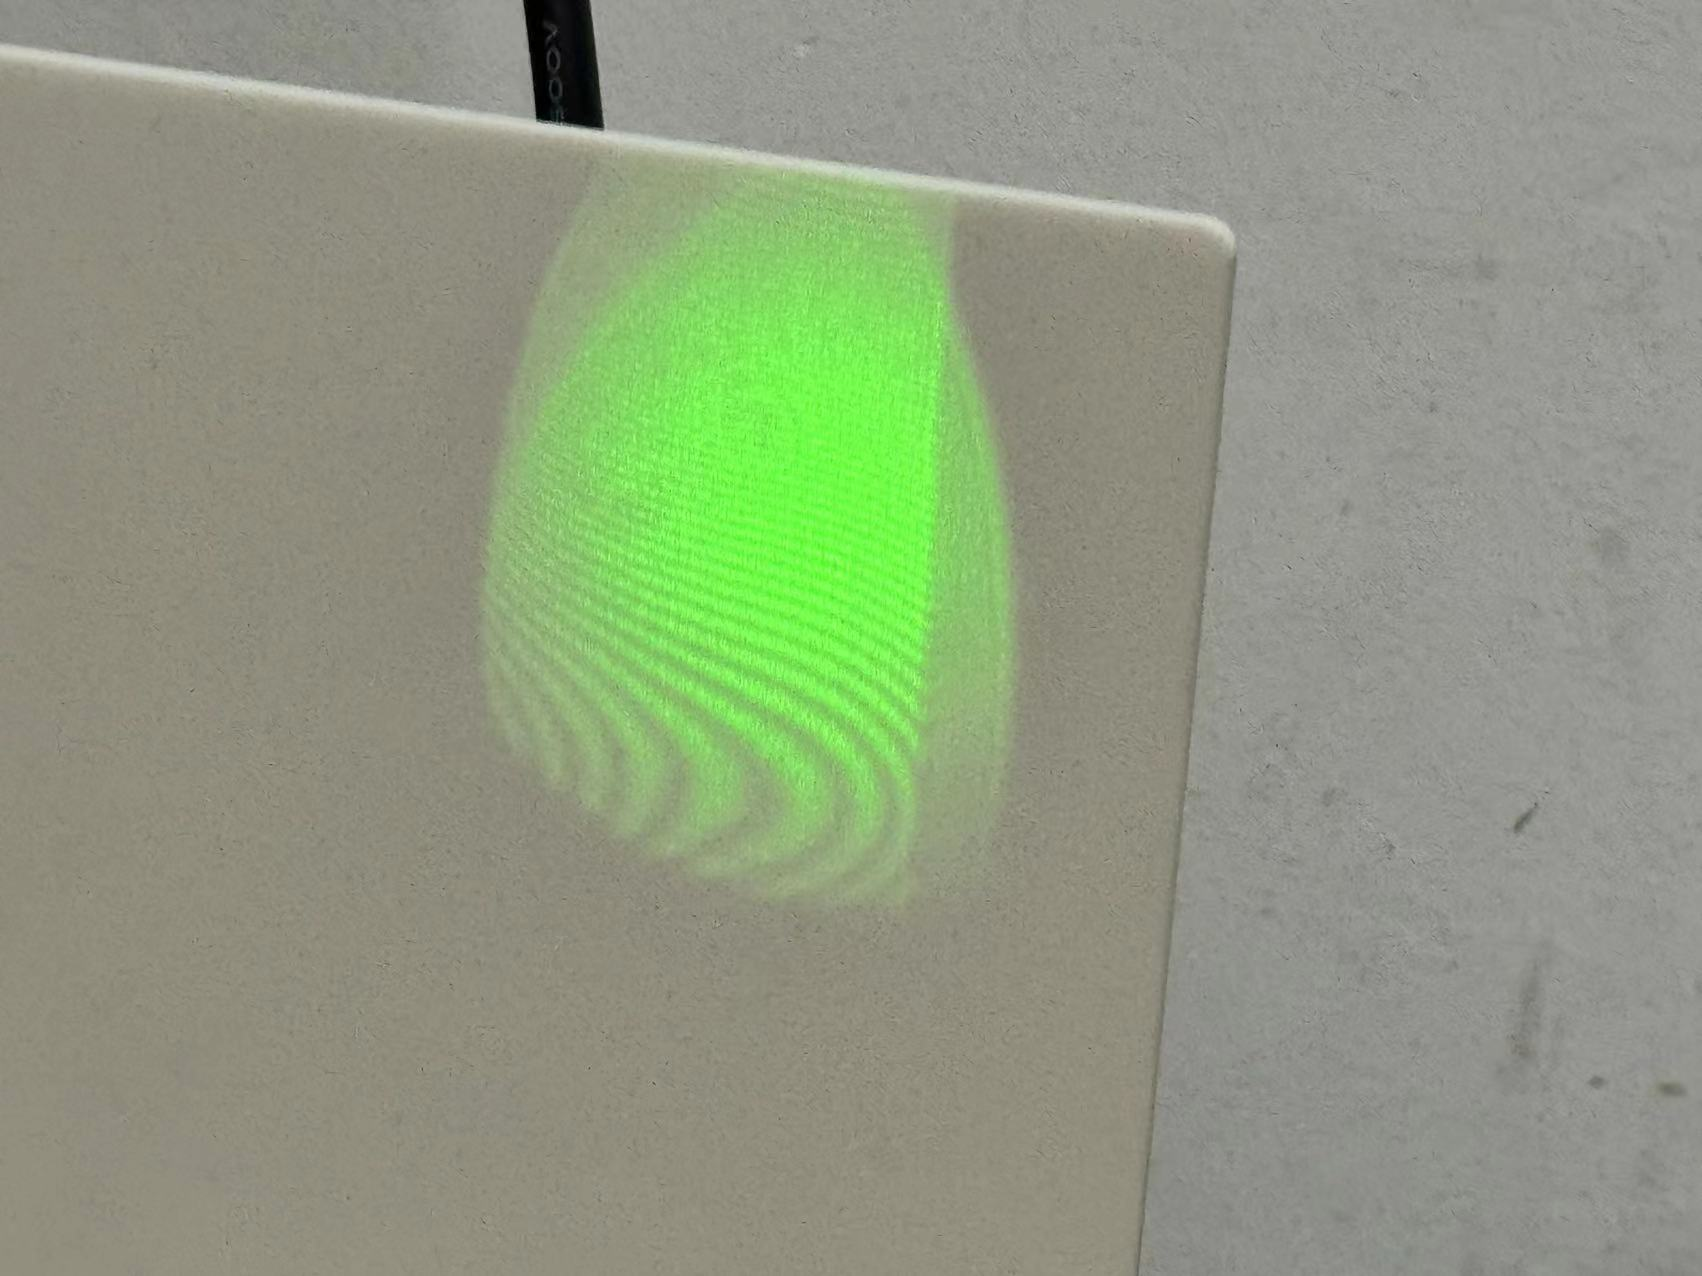
\includegraphics[width=0.8\textwidth]{其二.jpg}
    \captionof{figure}{调出的其他图案}
\end{minipage}
\section{实验心得}
\paragraph{总}在此次实验中,为了总结经验和加深影响,我们每个人都独立完成了一次完整的调节,且都调出了干涉图样,现在下面列出我们每位同学的心得感受。
\paragraph{此实验需要控制好每个调节自由度}在第一次调节时我们并未顾忌太多,认为只要最后一块镜子安放的位置正确就一定能产生干涉条纹,但却忽略了这两束光在空间上甚至并不一定相交。两束光从第一块分束镜分开后就分别被两个反射镜反射向不同的方向,且这两竖光走的完全独立,没有参照的路线(与迈克尔孙干涉仪相比,迈克尔孙干涉仪可反复利用干涉锁定光路),所以仅靠最后一块半透半反镜调节不可能产生出干涉条纹。
\paragraph{需要保证光线水平}如前所述,由于自由度的增加,若只考虑光线在水平面上的投影,很可能得不到最终的现象。体现在具体调节上,我们可以在开始实验时仔细调节激光器水平,可以确保在后续调节中不会因为光线不水平而产生的问题(比如最后两束光线没能成功“会和”)。
\paragraph{激光器相干长度短}此激光器的相干长度很短,我们必须将两个光路的长度调节到几乎完全相同。这也就意味着两条光路要尽可能垂直,在45度角的判断上目测十分困难,因此我们在调节时设法让每段光路在水平面上的投影都正好落在实验台的定位点所确定的直线上。这个调节是实验的关键步骤。
\paragraph{水平垂直调节}如前所述,实验中需要多次判断光路的方向是否水平以及是否与底座的定位点连线平行,因此必须使用到校准工具。移动校准工具时,保证其高度不变是很容易的,但是保证其在移动方向始终不变却比较困难。为此,可利用暂时没有用到的光具座,将校准工具沿着该光具座的一侧移动,如同制作了一个简易导轨。这样便可以方便观察光点的运动来使调节精确。
\paragraph{分束器调节技巧}为达到上述条件,我们需要反复调节分束器。这是一个二自由度的调节,我们要在反射点落在定位点上的同时把角度调节好,而在转动镜面时转轴又有可能并没有落在定位点上——这意味着我们要通过多次来回调节来达到这两个目标,我们可以把它类比为在交流电桥实验中为了使电桥尽量平衡而反复对各元件参数进行调节。在本实验中,我们使用定位光线的毛玻璃来辅助调节。毛玻璃离镜面较远时调节镜面角度,毛玻璃离镜面较近时调节底座位置,反复六七次左右即可完成调节。
\paragraph{关于出现的平行细条纹}在实验中很难做到两个光束的路径完全垂直,也就是在光屏上两个光束并不能完全形成等倾干涉,因此角度产生偏差,简化为两个夹角为$\theta$的平面波在光屏上发生干涉。故$I=I_0\cos^2(\frac{\pi \Delta x\sin\theta}{\lambda})$,从而产生平行细干涉条纹。
\end{document}